\documentclass[a4paper,12pt]{article} % добавить leqno в [] для нумерации слева
\usepackage[a4paper,top=1.3cm,bottom=2cm,left=1.5cm,right=1.5cm,marginparwidth=0.75cm]{geometry}
%%% Работа с русским языком
\usepackage{cmap}					% поиск в PDF
\usepackage{mathtext} 				% русские буквы в фомулах
\usepackage[T2A]{fontenc}			% кодировка
\usepackage[utf8]{inputenc}			% кодировка исходного текста
\usepackage[english,russian]{babel}	% локализация и переносы

\usepackage{graphicx}

\usepackage{wrapfig}
\usepackage{tabularx}

\usepackage{hyperref}
\usepackage[rgb]{xcolor}
\hypersetup{
colorlinks=true,urlcolor=blue
}
\usepackage{multirow}
\usepackage{hhline}


%%% Дополнительная работа с математикой
\usepackage{amsmath,amsfonts,amssymb,amsthm,mathtools} % AMS
\usepackage{icomma} % "Умная" запятая: $0,2$ --- число, $0, 2$ --- перечисление

%% Номера формул
\mathtoolsset{showonlyrefs=true} % Показывать номера только у тех формул, на которые есть \eqref{} в тексте.

%% Шрифты
\usepackage{euscript}	 % Шрифт Евклид
\usepackage{mathrsfs} % Красивый матшрифт

%% Свои команды
\DeclareMathOperator{\sgn}{\mathop{sgn}}

%% Перенос знаков в формулах (по Львовскому)
\newcommand*{\hm}[1]{#1\nobreak\discretionary{}
{\hbox{$\mathsurround=0pt #1$}}{}}

\begin{document}
	
	\begin{titlepage}
	\begin{center}
		{\large МОСКОВСКИЙ ФИЗИКО-ТЕХНИЧЕСКИЙ ИНСТИТУТ (НАЦИОНАЛЬНЫЙ ИССЛЕДОВАТЕЛЬСКИЙ УНИВЕРСИТЕТ)}
	\end{center}
	\begin{center}
		{\large Физтех-школа электроники, фотоники и молекулярной физики}
	\end{center}
	
	
	\vspace{4.5cm}
	{\huge
		\begin{center}
			{Лабораторная работа 2.2.1}\\
			Исследование взаимной диффузиии газов
		\end{center}
	}
	\vspace{2cm}
	\begin{flushright}
		{\LARGE Салтыкова Дарья \\
			\vspace{0.5cm}
			Б04-105}
	\end{flushright}
	\vspace{8cm}
	\begin{center}
		Долгопрудный 2022
	\end{center}
\end{titlepage}

\section{Введение}

\noindent
\textbf{Цель работы:} 1) регистрация зависимости концентрации гелия в воздухе от времени с помощью датчиков теплопроводности при разных начальных давлениях смеси газов; 2) определение коэффициента диффузии по результатам измерений.
\medskip

\noindent \textbf{Оборудование:} измерительная установка; форвакуумный насос; баллон с газом (гелий); манометр; источник питания; магазин сопротивлений; гальванометр; компьютерное ПО.

\medskip

\section{Теоретические сведения}

\medskip

\noindent Диффузией называют самопроизвольное взаимное проникновение веществ друг в друга, происходящее вследствие хаотичного теплового движения молекул. При перемешивании молекул разного сорта говорят о взаимной (или концентрационной) диффузии.

\medskip

\noindent Диффузия в системе, состоящей из двух компонентов $ a $ и $ b $ (бинарная смесь), подчиняется закону Фика: плотности потока компонентов $ j_{a,b} $ (количество частиц, пересекающих единичную площадку в единицу времени) пропорциональны градиентам их концентраций $ \nabla n_{a,b}$, что в одномерном случае можно записать как

\[ j_a = -D\frac{\partial n_a}{\partial x}, \quad j_b = -D\frac{\partial n_b}{\partial x}, \]

\noindent где $ D $ -- коэффициент взаимной диффузии компонентов. Знак <<минус>> отражает тот факт, что диффузия идёт в направлении выравнивания концентраций. Равновесие достигается при равномерном распределении вещества по объёму сосуда ($ \partial n / \partial x = 0 $).

\medskip

\noindent В данной работе исследуется взаимная диффузия гелия и воздуха. Давление P и температура T в условиях опыта предполагаются неизменными: $ p=(n_{He}+n_{\text{в}})kT $, где $ n_{He} $ и $ n_{\text{в}} $ -- концентрации (объёмные плотности) диффундирующих газов. Поэтому для любых изменений концентраций справедливо $ \Delta n_{He}=-\Delta n_{\text{в}} $. Следовательно, достаточно ограничиться описанием диффузии одного из компонентов, например гелия $ n_{He} $:

\begin{equation}\label{1}
j_{He}=-D\frac{\partial n_{He}}{\partial x}.
\end{equation}

\noindent Приведём теоретическую оценку для коэффициента диффузии. В работе концентрация гелия, как правило, мала $ (n_{He} \ll n_\text{в}) $. Кроме того, атомы гелия существенно легче молекул, составляющих воздух ($ \mu_{He} \ll \mu_{O_2}, \mu_{N_2} $), значит и их средняя тепловая скорость велика по сравнению с остальными частицами. Поэтому перемешивание газов в работе можно приближенно описывать как диффузию примеси лёгких частиц $ He $ на практически стационарном фоне воздуха. Коэффициент диффузии в таком приближении равен

\begin{equation}\label{2}
D=\frac{1}{3}\lambda \overline{v},
\end{equation}

\noindent где $ \overline{v}=\sqrt{\frac{8RT}{\pi \mu}} $ -- средняя тепловая скорость частиц примеси, $ \lambda = \frac{1}{n_0\sigma} $ -- их длина свободного пробега, $ n_0 $ -- концентрация рассеивающих центров (фона), $ \sigma $ -- сечение столкновения частиц примеси с частицами фона.

\medskip

\noindent Таким образом, теория предсказывает, что коэффициент диффузии бинарной смеси обратно пропорционален давлению в системе $ D \propto 1/P $, и не зависит от пропорций компонентов, что и предлагается проверить в работе экспериментально.

\medskip

\section{Схема эксперимента}

\medskip

\noindent Для исследования взаимной диффузии газов и измерения коэффициента взаимной диффузии $ D $ используется два сосуда объёмами $ V_1 $ и $ V_2 $ $ (V_1\approx V_2=V) $, соединенные трубкой длины $ L $ и сечения $ S $ (рис. 1). 

\medskip

\noindent Предполагается, что сосуды заполнены смесью двух газов при одинаковом давлении, но с различной концентрацией компонентов. Вследствие взаимной диффузии, проходящей в соединительной трубке, концентрации компонентов в сосудах с течением времени выравниваются. 

\medskip

\begin{wrapfigure}{r}{3.5cm}
	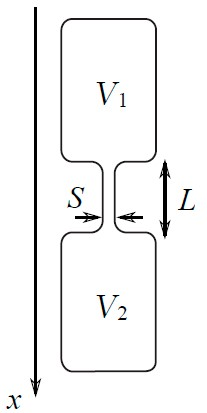
\includegraphics[width=3.5cm]{схема.jpg}
	\caption{Общая схема установки}
	\label{ris1}
\end{wrapfigure}

\medskip

\noindent Важно отметить, что диффузия -- относительно медленный процесс, и для его наблюдения необходимо отсутствие конвекции, т. е. макроскопических течений газа. Для этого необходимо обеспечить равенство давлений и температур в сосудах до начала измерений.

\medskip

\noindent В общем случае концентрации компонентов $ n(t, x) $ зависят от как от координаты, так и времени. Задача упрощается, если объём соединительной трубки мал по сравнению с объёмами сосудов -- тогда концентрации газов $ n_1(t) $ и $ n_2(t) $ внутри каждого сосуда можно считать постоянными по всему объёму сосуда, и принять, что процесс выравнивания концентраций происходит благодаря диффузии в трубке.

\medskip

\noindent Рассмотрим подзадачу о диффузии в соединительной трубке. Предположим сперва, что концентрации примеси (гелия) на её торцах поддерживаются постоянными и равными $ n_1 $ и $ n_2 $ соответственно. Тогда через некоторое время в трубке установится стационарный поток частиц, одинаковый в каждом сечении трубки (в противном случае, если бы поток зависел от $ x $, частицы бы накапливались в трубке, и процесс перестал бы быть стационарным). Применяя закон Фика в трубке, получим

\[ j=-D\frac{\partial n}{\partial x} = const \]

\noindent Следовательно, распределение концентрации в трубке $ n(x) $ -- линейная
функция:

\begin{equation}\label{3}
n(x) = \frac{\Delta n}{L} x
\end{equation}
и плотность потока частиц всюду постоянна и равна

\begin{equation}\label{4}
j=-D\frac{\Delta n}{L},
\end{equation}
\noindent где $ \Delta n = n_2-n_1 $ -- разность концентраций гелия на концах трубки.

\medskip

\noindent Теперь вернёмся к процессу выравнивания концентраций в сосудах. Частицы перетекают из сосуда 2 в сосуд 1 по трубке и концентрации $ n_1(t) $ и $ n_2(t) $ меняются во времени. Предположим, что этот процесс происходит достаточно медленно, так что в трубке в любой момент времени успевает установиться практически стационарное течение, описываемое формулами (1), (2). Такое приближение называют квазистационарным. Кроме того, будем считать, что в пределах каждого сосуда частицы распределены равномерно, так что концентрации примеси вблизи трубки и в остальных частях сосуда отличаются мало. Тогда полное число частиц примеси в сосудах равно соответственно $ N_1=n_1V $ и $ N_2=n_2V $. Произведение плотности потока (2) на площадь сечения трубки $ S $ даёт количество частиц, пересекающих в единицу времени любое поперечное сечение трубки. Поэтому

\begin{equation}\label{5}
\frac{dN_1}{dt}=jS, \quad \frac{dN_2}{dt}=-jS.
\end{equation}

\noindent Выразим отсюда скорость изменения $ \Delta n $. Вычитая из второго равенства первое и деля результат на объём сосуда $ V $, с учетом (2) получим

\begin{equation}\label{6}
\frac{d(\Delta n)}{dt}=-\frac{\Delta n}{\tau},
\end{equation}

\noindent где введено обозначение
\begin{equation}\label{7}
\tau=\frac{1}{D}\frac{VL}{2S}.
\end{equation}

\noindent Интегрируя (3), получаем, что разность концентраций будет убывать по экспоненциальному закону

\begin{equation}\label{8}
\Delta n = \Delta n_0 e^{-t/\tau},
\end{equation}

\noindent где $ \Delta n_0 $ -- разность концентраций примеси в сосудах в начальный момент времени. Видно, что величина $ \tau $ есть характерное время выравнивания концентраций между сосудами. Оно определяется геометрическими размерами установки и коэффициентом диффузии.

\medskip

\noindent Отметим, что для применимости квазистационарного приближения необходимо убедиться, что время процесса $ \tau $ много больше характерного времени диффузии отдельной частицы вдоль трубки $ L $, которое согласно закону Эйнштейна–Смолуховского по порядку величины равно

\begin{equation}\label{9}
\tau_\text{диф} \sim L^2/2D.
\end{equation}

\noindent Кроме того, если сосуды расположены вертикально, может возникнуть вопрос о влиянии силы тяжести на диффузию. Влиянием гравитации можно пренебречь, если перепад потенциальной энергии в сосуде много меньше энергии теплового движения частиц $ mgh \ll kT $. Нетрудно проверить, что для молекулярной диффузии в нашем эксперименте это выполняется с большим запасом.

\medskip

\section{Методика измерений}

\medskip

\noindent Для измерения разности концентраций в установке применяются датчики теплопроводности. При этом используется тот факт, что теплопроводность $ \kappa $ смеси зависит от её состава. В общем случае зависимость $ \kappa(n) $ довольно сложна, однако при малой разности $ \Delta n $ концентраций в сосудах можно ожидать, что разность теплопроводностей будет изменяться прямо пропорционально $ \Delta n $:

\[ \Delta \kappa = \kappa(n_2)-\kappa(n_1)\approx\text{const}\cdot\Delta n. \]

\noindent Эксперименты показывают, что если доля примеси гелия составляет менее 15\%, отклонение от линейной зависимости не превышает 0,5\%, что для наших целей вполне достаточно.

\medskip

\noindent Сами датчики теплопроводности устроены следующим образом. Тонкая платиновая проволочка, протянутая вдоль оси стеклянного цилиндра, нагревается током. Внутренняя полость датчика сообщается с объёмом камеры через отверстия, размеры которых таковы, что скорость диффузии из объёма сосуда в полость датчика значительно больше скорости диффузии из одного объёма в другой. Таким образом, состав газа в датчике практически совпадает с составом газа в объёме. Тепло от проволочки к стенке цилиндра передаётся главным образом за счёт теплопроводности газа, находящегося внутри цилиндра. При заданной мощности нагревания приращение температуры проволочки и, следовательно, приращение её сопротивления пропорциональны теплопроводности газа.

\medskip

\noindent Для измерения сопротивлений используется мостовая схема, позволяющая определять разность показаний датчиков с высокой точностью. Мост балансируется при заполнении сосудов (и датчиков) одной и той же смесью. При заполнении сосудов смесями различного состава возникает <<разбаланc>> моста. При незначительном различии в составах смесей показания вольтметра, подсоединённого к диагонали моста, будут пропорциональны разности концентраций примеси: $ U\propto\Delta\kappa\propto\Delta n $. В процессе диффузии разность концентраций убывает по закону \eqref{8}, и значит по тому же закону изменяется напряжение:

\begin{equation}\label{10}
U=U_0e^{-t/\tau},
\end{equation}

\noindent где $ U_0 $ -- показание гальванометра в начальный момент времени. Измеряя экспериментально зависимость $ U(t) $, можно получить характерное время
процесса $ \tau $, откуда по формуле \eqref{7} определить коэффициент диффузии $ D $.

\section{Экспериментальная установка}

\begin{figure}[h]
\center{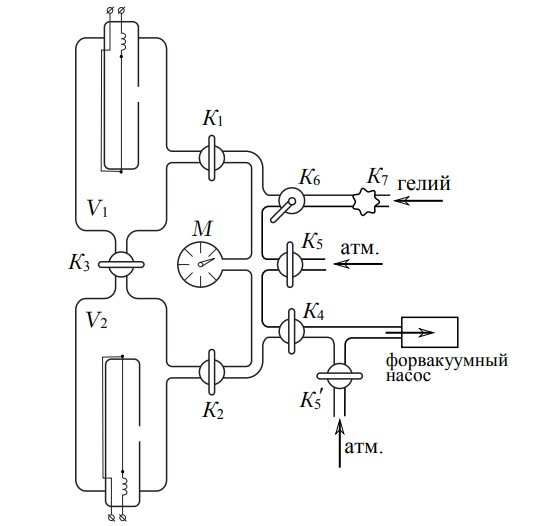
\includegraphics[scale={1.2}]{установка.jpg}}
\caption{Экспериментальная установка.}
\end{figure}


\noindent Схема установки приведена на рисунке. Измерительная часть соединена с системой откачки и напуска воздуха и гелия. Для откачки используется форвакуумный насос.

\medskip

\noindent Установка компьютеризирована, что позволяет записывать зависимость показаний вольтметра $ U(t) $ в реальном времени.

\medskip

\noindent Измерительная часть установки состоит из двух сосудов $ V_1 $ и $ V_2 $, размещённых вертикально. Краны $ K_1 $ и $ K_2 $ служат для управления откачкой и подачей воздуха/гелия в сосуды. Диффузия осуществляется через тонкую короткую трубку, соединяющую сосуды, оснащённую краном $ K_3 $. К соединительным трубкам подключен манометр M, измеряющий разность давлений между соединительными трубками и атмосферой, и позволяющий измерять давления в разных частях системы (в зависимости от положения кранов).

\medskip

\noindent Выравнивание давлений в сосудах $ V_1 $ и $ V_2 $ без изменения состава газов в них может быть осуществлено через обводные трубки посредством кратковременного открытия кранов $ K_1 $ и $ K_2 $ (при закрытом $ K_3 $).

\begin{wrapfigure}{r}{5cm}
	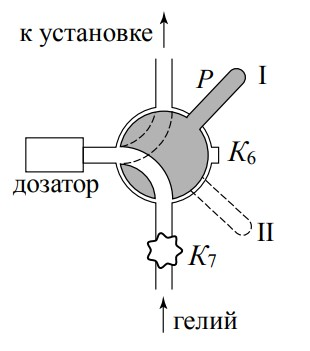
\includegraphics[width=5cm]{гелий.jpg}
	\caption{Механизм подачи гелия}
\end{wrapfigure}

\noindent Гелий содержится в баллоне под давлением, превышающим атмосферное. Для предотвращения избыточного расхода гелия и его неконтролируемого проникания в установку предусмотрен металлический кран $ K_7 $, отделяющий её от баллона с гелием. Его открывают только на время непосредственного заполнения установки гелием, остальное время он должен быть закрыт. Для подачи малых порций гелия предусмотрен двухходовый кран с дозатором (рис. 3). При повороте рычажка $ P $ в положение $ I $ гелий в небольшом количестве поступает в дозатор (если открыт $ K_7 $), а при повороте $ P $ в положение $ II $ порция из дозатора поступает в установку.

\medskip

\noindent Датчики теплопроводности Д$ _1 $ и Д$ _2 $, расположенные в сосудах $ V_1 $ и $ V_2 $ соответственно, включены в мостовую электрическую схему согласно рис. 4. В одну из диагоналей моста включён высокочувствительный вольтметр (гальванометр) Г, к другой подключается источник небольшого постоянного напряжения. Сопротивления проволок датчиков составляют одно из плеч моста. Второе плечо составляют переменные сопротивления $ R_1 $, $ R_2 $ и $ R $, служащие для установки показаний вольтметра Г на нуль (балансировка моста). Сопротивления $ R_1 $ и $ R_2 $ спарены (их подвижные контакты находятся на общей оси) и изменяются одновременно при повороте ручки грубой регулировки. Точная балансировка выполняется потенциометром $ R $. Балансировку необходимо проводить перед каждым экспериментом заново: при этом установка заполняется чистым газом (воздухом без гелия) при давлении, близком «рабочему» (при котором затем будут проводится измерения).

\begin{figure}[h]
	\begin{center}
		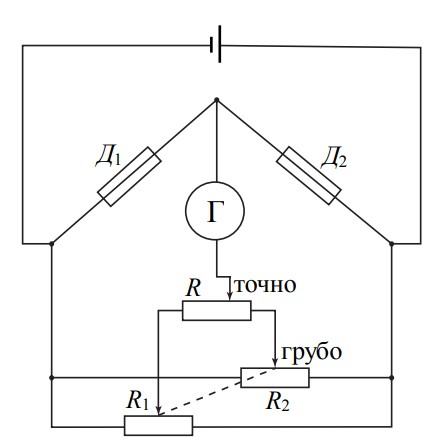
\includegraphics[width=7cm]{мост.jpg}
	\end{center}
	\caption{Мостовая схема}
\end{figure}

\section{Ход работы}

\medskip

\noindent 1. Подготовим установку к работе: сбалансируем мост, приготовим рабочие смеси.

\medskip

\noindent 2. Начнем процесс диффузии, открыв К3. Будем фиксировать показания вольтметра с течением времени с помощью компьютерной программы. Измерения будем продолжать до тех пор, пока напряжение не упадет на $50\%$. Повторим измерения при 5 различных значених рабочего давления.

\medskip

\noindent Результаты изобразим на графике в логарифмическом масштабе по оси ординат.

\medskip

\begin{figure}[h!]	\center{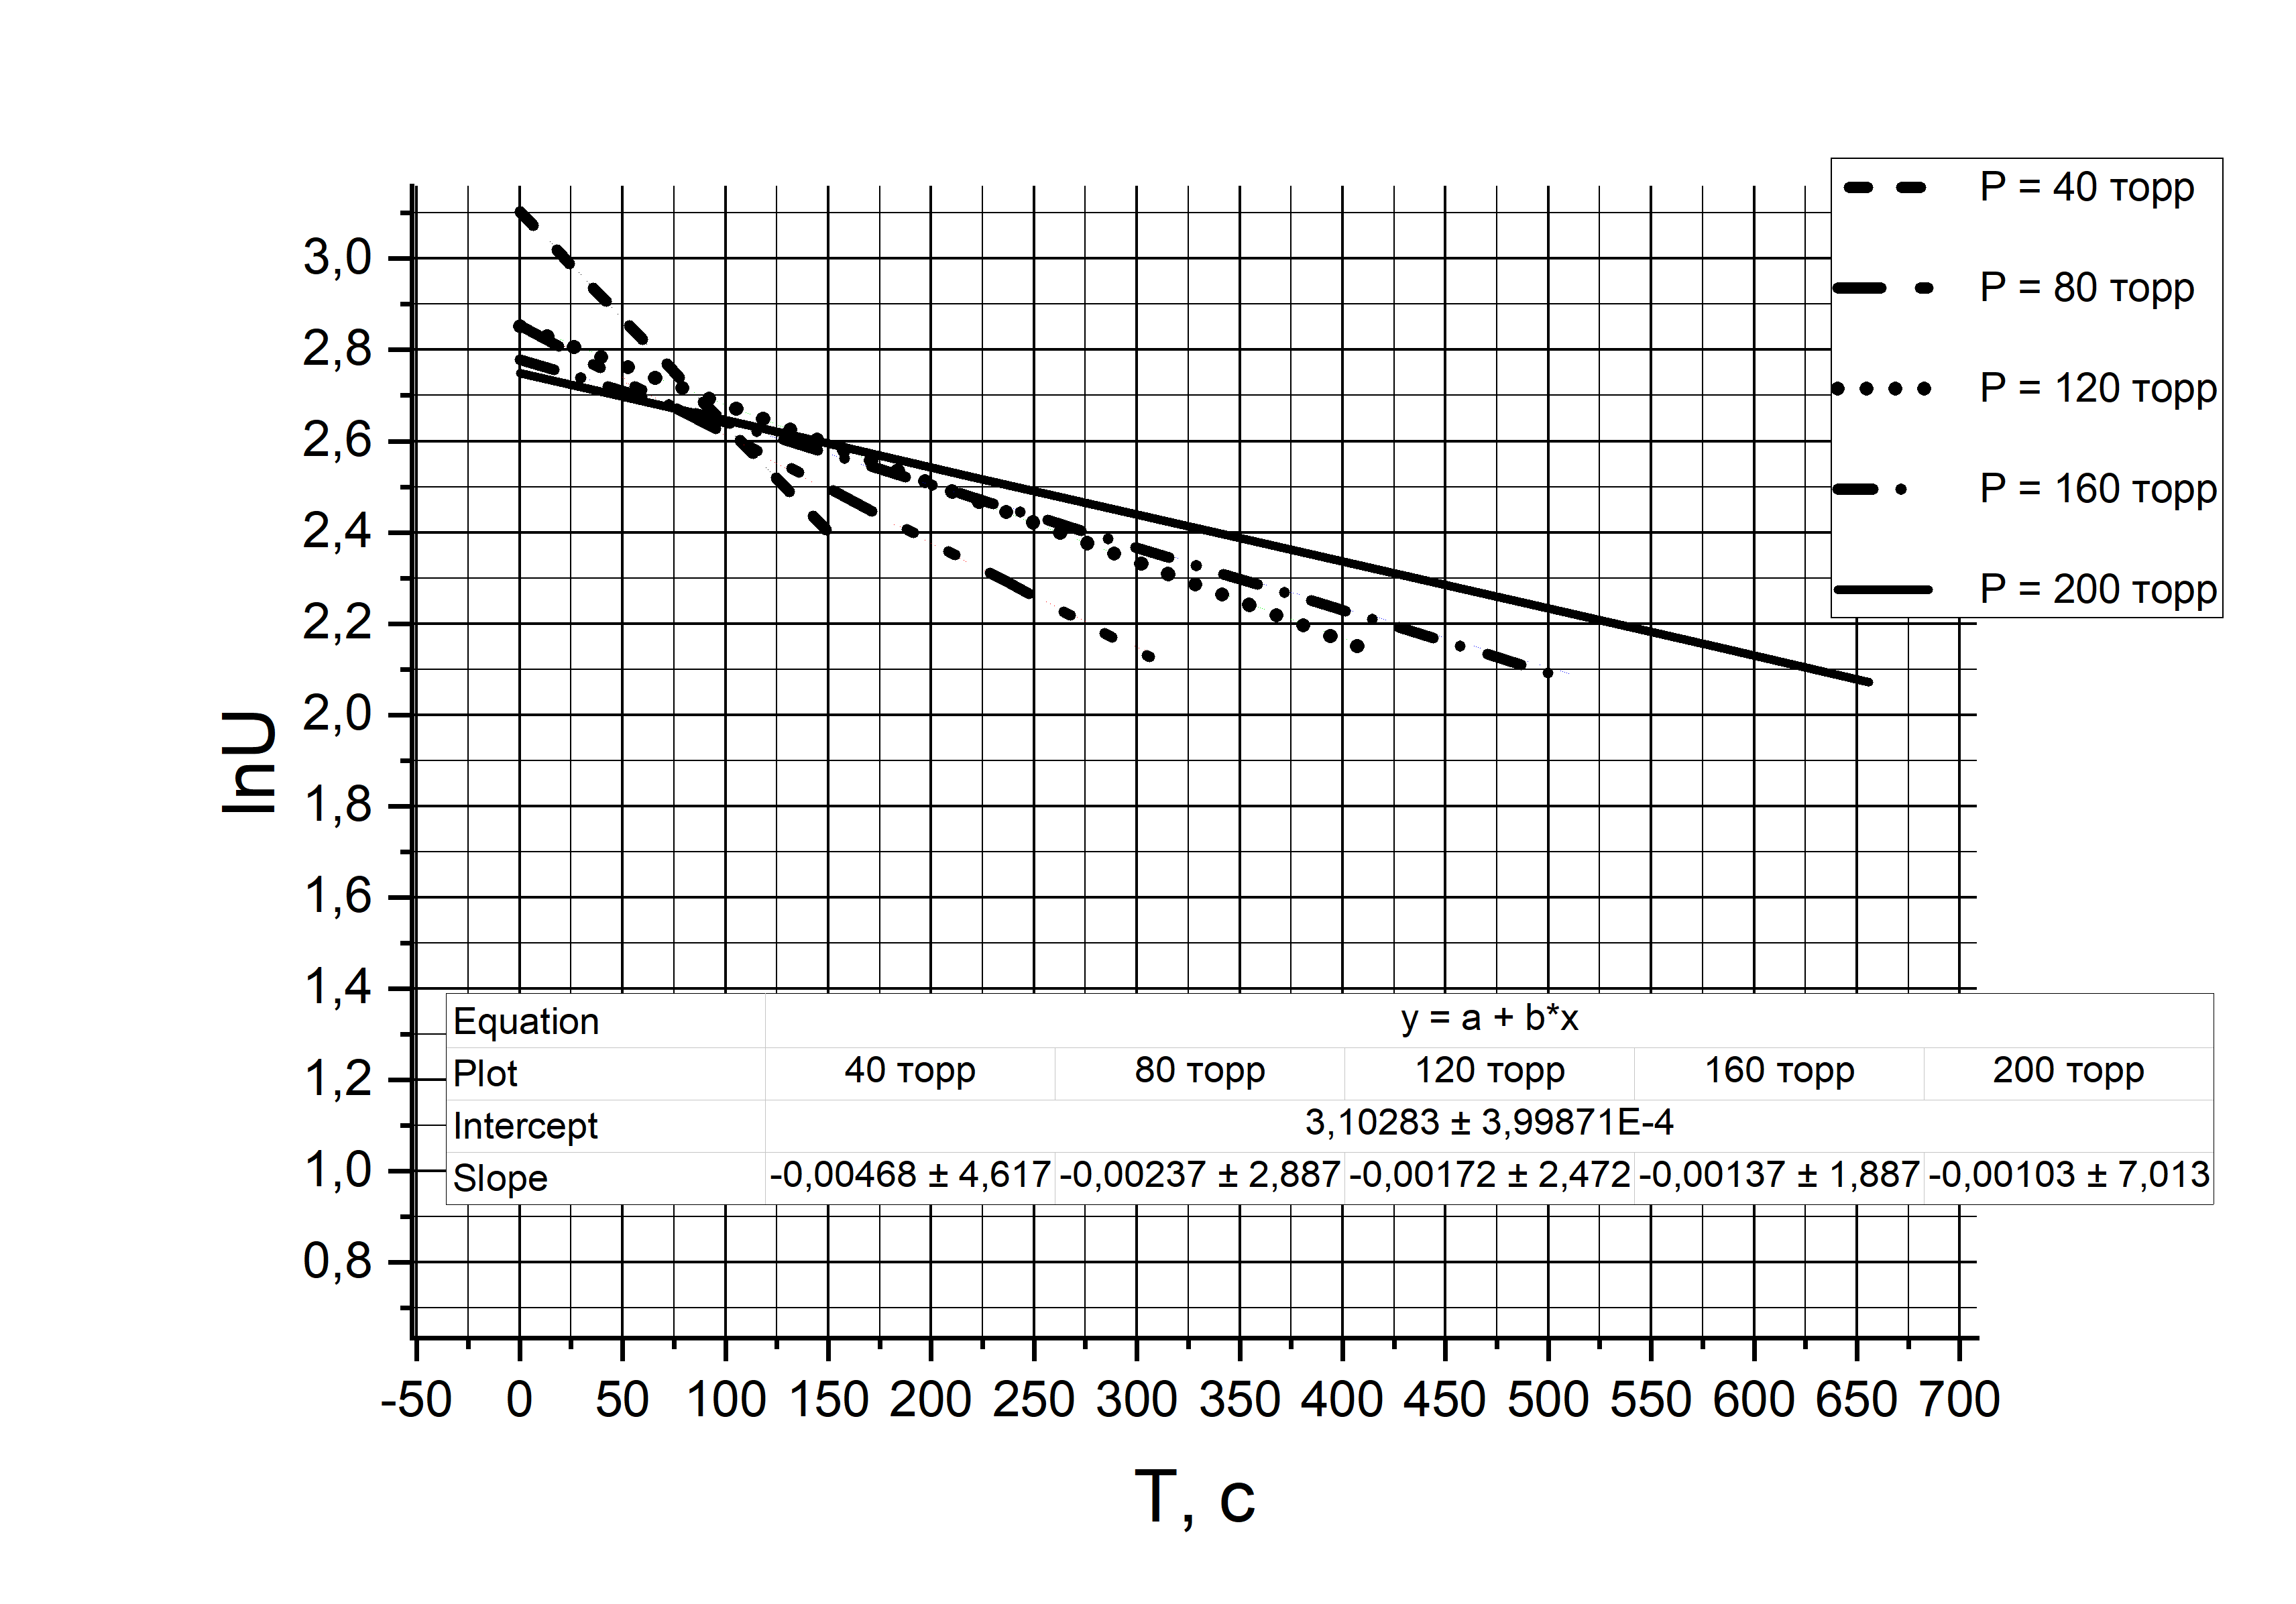
\includegraphics[scale=0.6]{1}}
\end{figure}
	
\noindent 3. Согласно формуле $U = U_0e^{-t/\tau}$, коэффициент b в уравнении прямой $y = ax + b$ на графике равен: 

\[ b = -\tau^{-1} \Rightarrow \tau = -b^{-1}. \]

\[ \sigma_\tau = \tau \cdot \frac{\sigma_{b}}{|b|}. \]

\noindent Расчитаем коэффициенты взаимной диффузии по формуле (1) и занесем результаты в таблицу. 

\medskip

\noindent Геометрические параметры установки:

\[ V = (1200\pm 30) \text{ см}^3,\] \[ \frac{L}{S} = (5,5 \pm 0,5) \text{ см}^{-1}. \]

\noindent Погрешность вычисление коэффициента взаимной диффузии по \eqref{D} можно оценить по следующей формуле:

\[ \sigma_D = D\sqrt{\left(\frac{\sigma_\tau}{\tau}\right)^2+\left(\frac{\sigma_V}{V}\right)^2+\left(\frac{\sigma_{L/S}}{(L/S)}\right)^2}. \]

\noindent Реузльтаты вычислений занесем в таблицу.

\medskip

\begin{tabular}{|c|c|c|c|c|c|c|c|}
\hline 
$P, \text{торр}$ & $\sigma_P, \text{торр}$ & $b, \cdot 10^{-3} {\text{с}}^{-1}$ & $\sigma_b, \cdot 10^{-3} {\text{с}}^{-1}$ & $\tau, \text{с}$ & $\sigma_\tau, \text{с}$ & $D, \frac{{\text{см}}^2}{\text{c}}$ & $\sigma_D, \frac{{\text{см}}^2}{\text{c}}$ \\ 
\hline 
40 & 2 & -4,68 & 0,0046 & 213,7 & 0,2 & 15,4 & 1,46 \\ 
\hline 
80 & 2 & -2,37 & 0,0029 & 421,9 & 0,5 & 7,80 & 0,74 \\ 
\hline 
120 & 2 & -1,72 & 0,0025 & 581,4 & 0,8 & 5,70 & 0,54 \\ 
\hline 
160 & 2 & -1,37 & 0,019 & 729,9 & 10,1 & 4,50 & 0,43 \\ 
\hline 
200 & 2 & -1,03 & 0,0007 & 970,9 & 0,7 & 3,40 & 0,32 \\ 
\hline 
\end{tabular} 

\medskip

\noindent 4. Построим график зависимости коэффициента диффузии от обратного давления в координатах $D(\frac{1}{P})$. 

\begin{figure}[h!]	\center{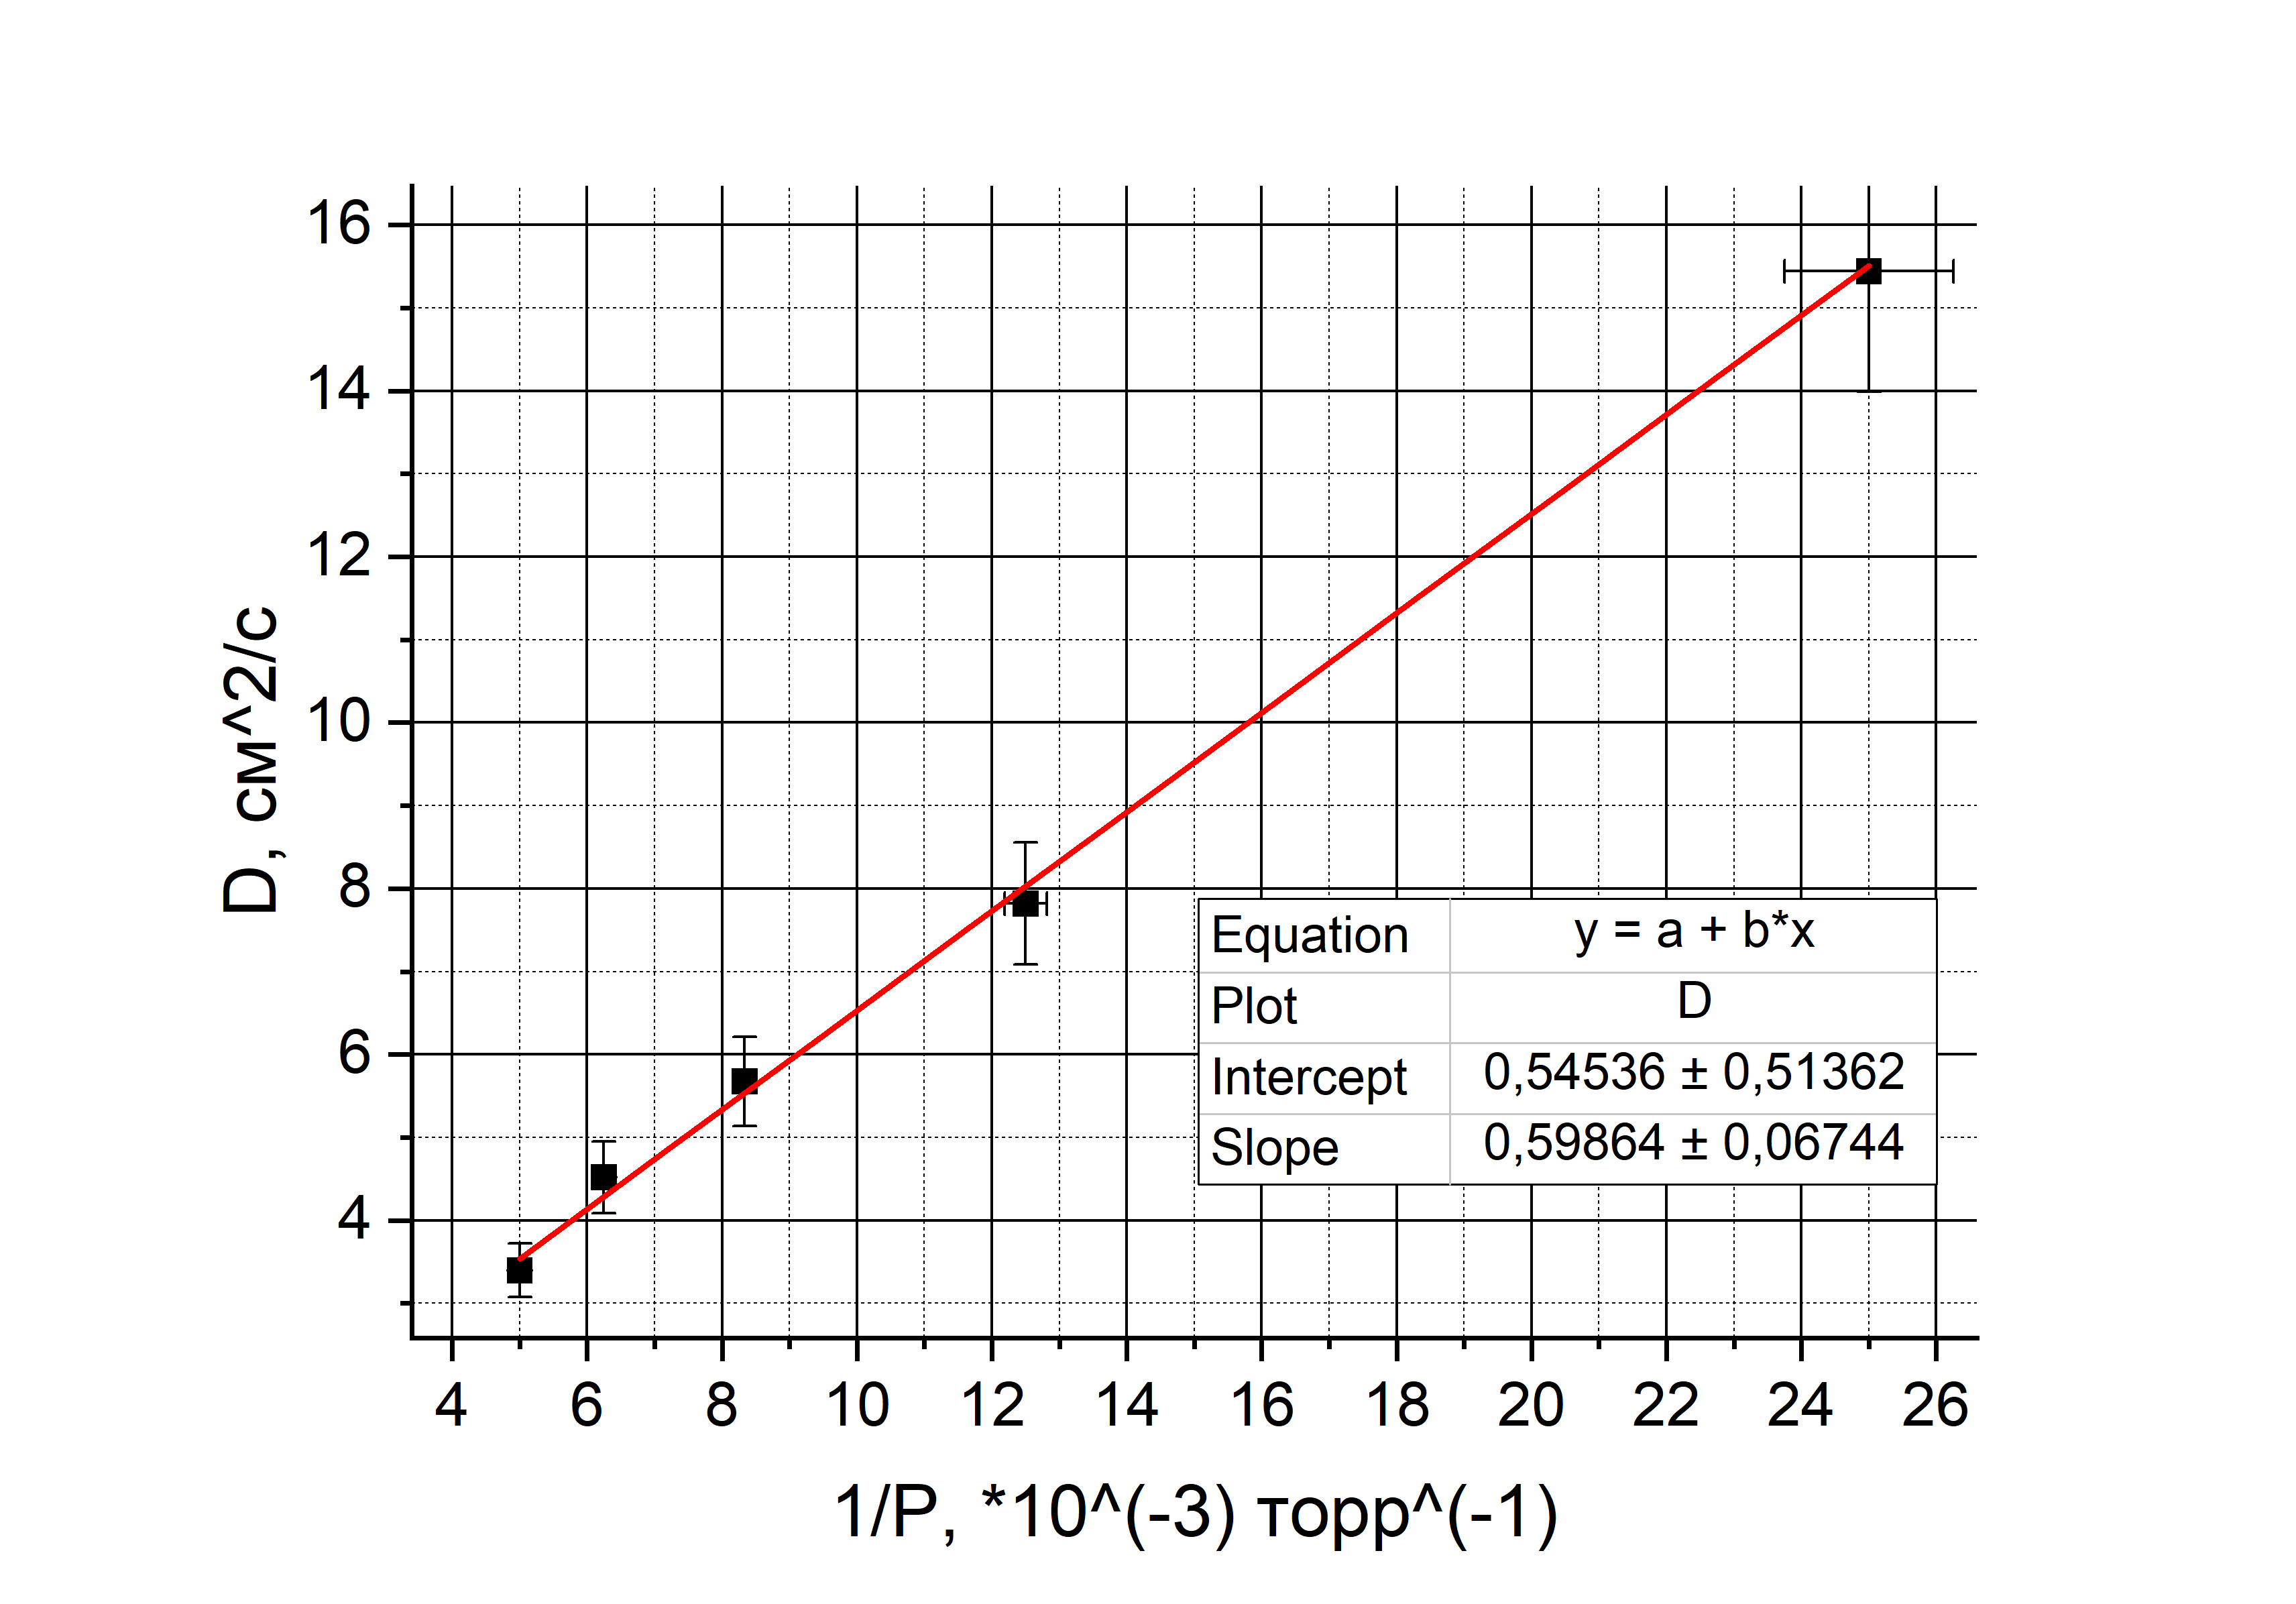
\includegraphics[scale=0.6]{2}}
\end{figure}
	

\medskip

\noindent Экстраполируя график к атмосферному
давлению ($ P=752 $ торр), оценим соответствующий коэффициент диффузии.

\[ D_\text{атм} = (0,54\pm0,05) \text{ } \frac{\text{см}^2}{\text{с}}. \] 

\medskip

\noindent 5. По полученным результатам оценим длину свободного пробега атомов
гелия в воздухе $\lambda_\text{He}$ в условиях эксперимента.

\[ D = \frac{1}{3}\lambda \overline{v} = \frac{1}{3}\lambda\sqrt{\frac{8RT}{\pi\mu}}. \]

\noindent Отсюда получаем следующее:

\[ \lambda = 3D\sqrt{\dfrac{\pi\mu}{8RT}} \approx (129 \pm 12) \text{ нм}.\]

\noindent Оценим эффективное сечение столкновений атомов гелия с молекулами воздуха $\sigma_\text{He-возд}$.

\[ \sigma_\text{He-возд} = \frac{1}{n_0\lambda}, \]

\noindent где $ n_0 = n_\text{He}+n_\text{возд}=\frac{P}{kT} = 2,44 \cdot 10^{25} $ м$ ^{-3} $ -- полная концентрация частиц. Получаем:

\[ \sigma_\text{He-возд} = (3,17 \pm 0,29) \cdot 10^{-19} \text{ м}^2}.\]


\section{Вывод}

\medskip

\noindent В ходе работы:

\begin{itemize}
	\item Был определён коэффициент взаимной диффузии для смеси гелий-воздух. Для атмосферного давления:
	
	\[ D_\text{атм} = (0,54\pm0,05) \text{ } \frac{\text{см}^2}{\text{с}}. \]
	
	Сравним полученное значение с табличным:

	\[ D_\text{табл} = 0,62 \text{ } \frac{\text{см}^2}{\text{с}}. \]

	\item Была оценена длина свободного пробега гелия в воздухе, а также эффективное сечение столкновения атомов гелия с молекулами воздуха.
	
	\[ \lambda = (129 \pm 12) \text{ нм}.\]
	
	\[ \sigma_\text{He-возд} = (3,17 \pm 0,29) \cdot 10^{-19} \text{ м}^2}.\]
	
	\noindent Табличные значения:
	
	\[ \lambda_\text{табл} = 175 \text{ нм}, \]

\[ \sigma_\text{табл} = 5,89  \cdot 10^{-19} \text{ м}^2.\]
	
\end{itemize}

\noindent Полученные экспериментально значения не совпадают с табличными в пределах погрешности, но соответствуют им по порядку величины.

\medskip

\noindent Основную погрешность в результаты внесло несовпадение рассчитываемого рабочего давления с тем, что получается после наполнения сосудов газами. 

\end{document}